\documentclass[11pt,a4paper]{ujreport} 	% for uplatex
%
\usepackage{amsmath,amssymb}
\usepackage{bm}
\usepackage{graphicx}
\usepackage{ascmac}
\usepackage{float}
\usepackage[dvipdfmx]{hyperref}
\usepackage{pxjahyper}
\hypersetup{% hyperrefオプションリスト
setpagesize=false,
 bookmarksnumbered=true,%
 bookmarksopen=true,%
 colorlinks=true,%
 linkcolor=blue,
 citecolor=red,
}

%
\setlength{\textheight}{40\baselineskip}
\addtolength{\textheight}{\topskip}
\setlength{\voffset}{-0.2in}
\setlength{\topmargin}{0pt}
\setlength{\headheight}{0pt}
\setlength{\headsep}{0pt}

\setlength{\textwidth}{\paperwidth}     % ひとまず紙面を本文領域に
\setlength{\oddsidemargin}{-5.4truemm}  % 左の余白を20mm(=1inch-5.4mm)に
\setlength{\evensidemargin}{-5.4truemm} % 
\addtolength{\textwidth}{-40truemm}     % 右の余白も20mmに
%
\newcommand{\divergence}{\mathrm{div}\,}  %ダイバージェンス
\newcommand{\grad}{\mathrm{grad}\,}  %グラディエント
\newcommand{\rot}{\mathrm{rot}\,}  %ローテーション
%
\title{脳波解析のための数学シリーズ\\
 解析編}
\author{後藤 優仁}
\date{\today}
\begin{document}
\maketitle
%
%
\tableofcontents
\newpage

\section{はじめに}

さて, 基礎を学んだところで, ここからはいよいよ理工系の学生, 脳というブラックボックスに挑む学生として学ぶべき, 高度(?)な数学に挑戦していきます.\\ 
 わくわくしますね!!!\\
 この書を理解する事が出来れば,脳波解析の基本は抑えられたといっても過言ではあるけどまあ一般の修士程度の知識はつけられると思います.
\chapter{フーリエ変換}
この章では脳波解析の初歩というか基本.フーリエ変換を学習していきます.基本中の基本というか,これがないと何も解析ができないので頑張りましょう.と言っても,材料は既にbasicの方で抑えてあるのであとはじゃんじゃん動かすだけです.
\section{オイラーの公式}
まずはオイラーの公式の導出からいきましょう!!!\\
\\
 今まで, 証明をずっと後回しにしてたくせによく使っていた理由は, まずこの公式の導出には様々な数学的知識が必要であることです. また, やや直感的に分かりにくい公式であるため, 導出より先にその利便性, 利用のされかたに触れて慣れてほしかったのです.\\
\\
改めて, オイラーの公式を眺めてみましょう.\\
\begin{eqnarray}
\mathrm{e}^{i\theta} = \cos\theta + i\sin\theta
\end{eqnarray}

しっかりと理解するため,まずはこいつをちょっと解剖してみましょう. 数学語を日本語に翻訳すると, おそらくこんな感じになります.
\\
\\
 指数関数 $\mathrm{e}^x$のxに角度$\theta$を代入し, 虚数単位$i$をかけたもの(左辺)が, $sin$ と $cos$ の足し算で表した何らかの値と同じ値を表している.\\
\\
 うーん謎ですね.\\
 なぜ指数関数が三角関数で表せるのか?\\
 三角関数の足し合わせってなんだよ?\\
 指数関数を虚数にするってなんだよ??\\
\\
 これらの疑問を解消するため,少しずつ見ていきましょう.
\subsection{マクローリン展開}
さて, 一旦オイラーの公式は忘れてみましょう.\\
\\
 大学で学ぶ数学, とりわけ微分積分において最初に我々が躓く単元に, テイラー展開・マクローリン展開がありますね!\\
\\
 オイラーの公式は, このマクローリン展開さえ分かれば一瞬で導出する事が可能です.\\
\\
 はじめに,テイラー展開とマクローリン展開の違いは, テイラー展開の限定された特殊形がマクローリン展開です. なのでマクローリン展開だけここでは扱います.\\
\begin{eqnarray}
f(x) = \sum_{k=0}^\infty f^{(k)} (0) \frac{x^k}{k!} = f(0) + f'(0)x + \frac{f''(0)}{2!}x^2 + \frac{f'''(0)}{3!}x^3 ...
\end{eqnarray}

これがマクローリン展開です.\\
 元関数f(x)を多項式で近似するわけですね.\\
\\
 ここで使われる多項式は, 元関数fのx=0の時の高階微分係数から定まっています.\\
\\
 こいつの凄いのは, 局所的なある一点での振る舞いだけをみれば元の関数がわかるって事です!!\\
 テイラー展開とは, この時のxの値が0じゃなくてどこでもいいってやつで, マクローリン展開はx=0に限ったやつの事です.\\
\\
 $x=0$の時に最も元関数っぽい一次関数, 二次関数, 三次関数...と$\infty$に足し合わす事で元関数を表そうって事です!!!\\
 便利そうですね. 計算はだるいが.\\
\subsection{指数関数と三角関数のマクローリン展開}
さて, ここで指数関数と三角関数(sin, cos)のマクローリン展開を見てみましょう!!\\

\begin{figure}[H]
\label{im:exp}
  \centering
  \includegraphics[width=12cm]{../figures/exp.eps}
  \caption{exp関数のマクローリン展開}
\end{figure}
\begin{figure}[H]
\label{im:sine}
  \centering
  \includegraphics[width=12cm]{../figures/sine.eps}
  \caption{sin関数のマクローリン展開}
\end{figure}

\begin{figure}[H]
\label{im:cosine}
  \centering
  \includegraphics[width=12cm]{../figures/cosine.eps}
  \caption{cos関数のマクローリン展開}
\end{figure}

\begin{eqnarray}
\mathrm{e}^x = \sum_{(k=0)}^\infty \frac{x^k}{x!} = 1 + \frac{x}{1!} + \frac{x^2}{2!} + \frac{x^3}{3!} + ...
\label{eq:sisuu}
\end{eqnarray}

\begin{eqnarray}
\sin x = \sum_{k=0}^{\infty}(-1)^k \frac{x^{2k + 1}}{(2k + 1)!} = \frac{x}{1!} - \frac{x^3}{3!} + \frac{x^5}{5!} - \frac{x^7}{7!} +  ...
\label{eq:sain}
\end{eqnarray}

\begin{eqnarray}
\cos x = \sum_{k=0}^\infty(-1)^k \frac{x^{2k}}{(2k)!} = 1 - \frac{x^2}{2!} + \frac{x^4}{4!} - \frac{x^6}{6!} + ...
\label{eq:cosa}
\end{eqnarray}

勘の良い人なら気付くでしょう.\\
 なんとなくですが, 式(\ref{eq:sain})と式(\ref{eq:cosa})を足すと, 式(\ref{eq:sisuu})っぽいですよね.\\
\\
 気になるので,どうにかいじって等号で結べないか確かめてみます.とりあえず足してみましょう.
\\
\begin{eqnarray}
\mathrm{e}^x = \sum_{(k=0)}^\infty \frac{x^k}{x!} = 1 + \frac{x}{1!} + \frac{x^2}{2!} + \frac{x^3}{3!} + \frac{x^4}{4!} + ...
\end{eqnarray}
\begin{eqnarray}
\sin x + \cos x = 1 + \frac{x}{1!} - \frac{x^2}{2!} - \frac{x^3}{3!} + \frac{x^4}{4!} + ...
\label{eq:mix}
\end{eqnarray}

やはり似ていますね. もうちょっと, あとは符号だけ変えちゃえばいけそうなのですが...\\
 2項ずつ, 符号があってたりあってなかったりしてますね.\\
\\
 これは一寸難しいですね. もし交互に異なるのであれば, 式(\ref{eq:mix})の構成要素のどちらかに -1 をかければ良いのですが, 2項ずつとなるとそうもいきません. かといって両方にマイナスをかけても, 違う形になるし...\\
\\
 しかしよく考えてみましょう.それぞれのはn乗になっています. なんとか乗した時に符号が変わればいいのですから, ここで虚数単位iの導入に目星をつけます.こいつは2乗すると$-1$になるんでしたね.\\
\\
 とりあえず指数の方にやってみましょう.

\begin{align}
\mathrm{e}^{ix} \\
& = \sum_{(k=0)}^\infty \frac{ix^k}{x!} = 1 + \frac{ix}{1!} + \frac{i^2x^2}{2!} + \frac{i^3x^3}{3!} + \frac{i^4x^4}{4!} + ...\\
& = 1 + i\frac{x}{1!} - \frac{x^2}{2!} - \frac{ix^3}{3!} + \frac{x^4}{4!} + ...
\label{eq:eix}
\end{align}

ちょっといい感じですね.\\
 次に, 分母が奇数の時にiが残ってしまっているので, 奇数に対応しているsinの方にもiをかけてみましょう!\\
\begin{eqnarray}
i\sin x = \sum_{k=0}^{\infty}(-1)^k \frac{ix^{2k + 1}}{(2k + 1)!} = \frac{ix}{1!} - \frac{ix^3}{3!} + \frac{ix^5}{5!} - \frac{ix^7}{7!} +  ...
\end{eqnarray}
 問題なさそうですね!改めてcosと足してみます!!\\
\begin{eqnarray}
\cos x + i\sin x = 1 + i\frac{x}{1!} - \frac{x^2}{2!} - \frac{ix^3}{3!} + \frac{x^4}{4!} + ...
\label{eq:cossin}
\end{eqnarray}
 式(\ref{eq:eix})と式(\ref{eq:cossin})を見比べると, 見事に一致しています!!!\\
\\
 これでオイラーの公式の証明がおわりですね.お疲れさまでした.\\
\\
 オイラーの公式とは, 指数関数と三角関数をマクローリン展開した際にでてきた奴らが似ていたので, 虚数を導入してみたらきれいに等号で結べたねって事です.\\

\subsection{オイラーの公式の有用性}
オイラーの公式とは
\begin{eqnarray}
\mathrm{e}^{i\theta} = \cos \theta + i\sin \theta
\end{eqnarray}
でした.\\
\\
 この時, $\theta$に$\pi$を代入すると, 更に美しくなります.
\\
\begin{eqnarray}
\mathrm{e}^{i\pi} = -1 + 0\\
\mathrm{e}^{i\pi} + 1 = 0
\end{eqnarray}
 実際に計算すれば分かりますね. たしかに成り立ちます. \\
 最も基本である数字0と1, そしてネイピア数, 円周率, 虚数...\\
 数学において偉大と言われる奴らが一堂に会して, あっさりとまとまっているのです!!!\\
 ひええええ...!!!\\
\\
 これこそが, オイラーの公式が人類の至宝といわれる所以です.とても綺麗ですね.\\
\\
 オイラーの公式はこのように,三角関数を実数と虚数で足し合わせた極座標表示した時,指数関数に変換できますよというものでした.この性質を使って,次節以降のフーリエ変換が行われます.

\section{フーリエ変換}
 さて, いよいよ本節から実際に我々が脳波と戦う際に用いる技の紹介となっていきます. 基礎 (basic.pdf) が理解できている諸君なら, それほどつまずく事もないはずです. 実際筆者は, これまでの内容の理解に非常に時間をかけましたが, これ以降はそれほど時間をかけずに理解を進める事が出来ました. 基本を忘れなければ大丈夫です.数式はどんどんいかつくなりますが,落ち着いて臨んでください.部分部分は既に知っている数式の組み合わせになっているはずです.
\subsection{脳波とは}
そもそも, 解析方法を考える以前に...\\
 我々は脳波という似非科学チックな香ばしいものと対峙するわけですが, こいつの特性を知らずに武器や魔法を準備するのは非効率ですね. まずは脳波というものがどういったものなのかを考えてみます. \\
\\
 脳波とは, 脳に無数に存在する脳神経細胞が刺激を受け, その総量が閾値を超えた時に発生される電気信号 ... の集合体みたいなものでしたね.分からない人はまずそっちを勉強してきてください.\\
\\
 領域Aに脳細胞が100万個あったとしましょう. \\
 そのうち, 70万個が発火していて, 30万個が沈黙していたとします. 領域A直上にある脳波計の電極は, そこら一帯の電気的活動の総和を観測し, 領域Aで強い活動があったと記すわけです(図\ref{im:topo}).\\
\\
 この時の「強い活動」というのは, 電極で計測された電気信号の振幅, 100万の細胞電位の総和の値です. これが大きい程, 強い活動という解釈がされます.\\

\begin{figure}[H]
\label{im:topo}
  \centering
  \includegraphics[width=8cm]{../figures/topomap.eps}
  \caption{電極で拾われる脳波のイメージ. 近傍電位の総和}
\end{figure}

 しかし, 元来神経細胞の1回の発火は一瞬のものです. 2つの細胞があったとして, それらが数ms間隔で交互に活動しているとしたら, 片方が発火している間にもう片方は負の方向に電位を発しているわけですから, その総和を取ると細胞1個の発火分にも満たない事になります. \\
 これは当然, 数百万単位の細胞が集まった時にも同じ事が言えて, 振幅が小さいからといって脳が活動していない ... という訳ではありません. 単に同期的活動を行っているわけではないという事です.\\
\\
 本来はパルス波っぽい挙動をする神経信号ですが, それらが無数に存在し, 各々のタイミングで活動をしているため, 脳波計の電極によって計測される総和信号は連続的で, 非常に複雑な挙動を取る波となります. \\
\\
 この波を俗に脳波と言い, 振幅が大きい時には強い活動 (正確には同期した活動) が行われていて, 逆に振幅が小さい時には同期していない, つまりばらばらな活動を行っているといった解釈がなされたりします. \\
 しかしこのままでは, 複雑すぎて人間の目で見たら何がどうなっているのか全く分からず, 麻酔科医やてんかんの診断をする超能力医者のようなスーパーマンでもない限り, 「これは○○の脳波だ!」とか言えません. そこで凡人の我々は, どうにかしてこの複雑怪奇な脳波を解釈し, 脳の活動を解明する必要があるわけです.\\

 そこで, 最も基礎となるアプローチが...\\
 複雑すぎて分からないなら, 単純な波に分解してあげればいいじゃん??\\ 
 というやつです. どんな波も, 直交性をもつ波に分解できるみたいな話題が基礎編にありましたよね?あれを利用します.
\\
 こうして, 複雑極まりない脳波を, 単純で解釈のしやすい三角関数の足し合わせとして表現しよう!というのがフーリエ変換のモチベーションです.\\

\begin{figure}[H]
\label{im:eeg}
  \centering
  \includegraphics[width=12cm]{../figures/eeg.eps}
  \caption{A. 脳波の例 1 ~ 4は周波数帯成分}
\end{figure}

\subsection{フーリエ級数展開}
さて, フーリエ変換をする目的は, 複雑すぎて解釈できない時間関数を単純な関数によって表現する事でした.\\
\\
 複雑な関数でも, 三角関数の足し合わせで表現できるという事は既に確認しましたね. 三角関数の特徴は, その振幅と角周波数だけで定義する事ができます. \\
 角周波数とは, 1sの間にどれだけの角度波が進むかという指標で, 周波数とかから求める事が出来ます. まあ周波数って考えちゃっても大体おkです. \\
\\
 つまりフーリエ変換とは, 複雑な元関数を単純な三角関数の足し合わせと考え, それぞれの振幅を角周波数毎に求める事をさします.\\
\\
 このうち, 元関数f(t)を単純な三角関数の足し合わせに分解するまでをフーリエ級数展開と言い, 式では以下のようになります. 
\begin{eqnarray}
f(t) = a_0 + \sum_{\omega=1}^\infty {(a_\omega \cos(\omega t) + b_\omega \sin(\omega t))}
\label{eq:fourierkyusu}
\end{eqnarray}

式(\ref{eq:fourierkyusu})の意味はこうです. 「元関数$f(t)$を, 1から$\infty$の角周波数$(\omega)$の$sin, cos$波の足し合わせとして表現する」 そのまんまですね!\\
\\
 ここでの$a$や$b$はその周波数の波の大きさを決める変数で, それぞれの項毎に異なる値を取ります. 要は振幅の事ですね.\\
\subsection{複素フーリエ級数}
しかし, 式(\ref{eq:fourierkyusu})は面倒ですね. なんていったってsinとcosを分けて計算するのがだるすぎます. どうにか綺麗にできないものか...\\
\\
 はい.そこでオイラーの公式を使うわけですね.
\begin{eqnarray}
\mathrm{e}^{i\omega t} = \cos\omega t + i\sin\omega t
\label{eq:normaleuler}
\end{eqnarray}
 いつもは$\pi$のところですが, 今回は空気を読んで角周波数$\omega t$に変形しています. 角周波数に時間をかけてるんだから,その時間$t$の時の角度です.\\
 しかし問題はあれです. オイラーの公式には$i$がありますが, フーリエ級数展開の方には$i$がありません. どうしたことか.\\
\\
 ここで少し裏技というか,オイラーの公式の裏を使います.
\begin{eqnarray}
\mathrm{e}^{-i\omega t} = \cos\omega t - i\sin\omega t
\label{eq:eulerminus}
\end{eqnarray}
 式(\ref{eq:eulerminus})が成り立つのは大丈夫ですね?角度が実軸対称に飛んだら, cos成分は変わりませんがsin成分は符号が反転します. うちの猫でも知ってる事です.\\
\\
 さて, 次に式(\ref{eq:normaleuler})と式(\ref{eq:eulerminus})を連立して解く事で式(\ref{eq:fourierkyusu})のcosとsinを置き換えます. \\
\begin{eqnarray}
f(t) = a_0 + \sum_{\omega=1}^\infty {(a_\omega \frac{\mathrm{e}^{i\omega t}+\mathrm{e}^{-i\omega t}}{2} + b_\omega \frac{\mathrm{e}^{i\omega t} - \mathrm{e}^{-i\omega t}}{2i})}
\label{eq:complexfourier}
\end{eqnarray}
 この式を同類項を抜き出して整理すると
\begin{eqnarray}
f(t) = a_0 + \sum_{\omega=1}^\infty {(\frac{a_\omega - ib_\omega}{2}\mathrm{e}^{i\omega t})} + \sum_{\omega=1}^\infty {(\frac{a_\omega + ib\omega}{2}\mathrm{e}^{-i\omega t})}
\label{eq:complexfourierkai}
\end{eqnarray}
となり, 更に$\mathrm{e}^{-i\omega t}$において$\omega$を1から$\infty$まで足すのと, $\mathrm{e}^{i\omega t}$において$-\infty$から-1まで足すのは同義なため(図を書けばわかる), この3項をうまくくっつける事で
\begin{eqnarray}
f(t) = \sum_{\omega = -\infty}^\infty F_\omega \mathrm{e}^{i\omega t}
\end{eqnarray}
とおけますね!いい感じにまとまりました!!!\\
 あ, 定数部分は面倒なので$F_\omega$とおいてます. \\
\\
 ここまでがフーリエ級数展開でした.フーリエ変換とは, この係数たちを求める作業のことを指します. 
\subsection{フーリエ変換} 
 実際に式を見てみましょう.\\
\begin{eqnarray}
F(\omega) = \int_{-\infty}^{\infty} f(t)\mathrm{e}^{-i\omega t} dt
\label{eq:furier}
\end{eqnarray}

です. さっそく式(\ref{eq:furier})を解読してみましょう. 大丈夫. 基礎がしっかりできている人なら自ずと理解できるはずです.\\
\\
 まず, eの肩に $ -i\omega t $ が載っていますね. この形はどこかで見た事があります. そう, オイラーの公式ですね!!\\
 オイラーの公式にマイナスをかけたやつです. つまり $ \cos\omega t  - i\sin\omega t $ ですね. \\
 なので式(\ref{eq:furier})は以下の式に変形できそうです.\\
\begin{eqnarray}
F(\omega) = \int_{-\infty}^{\infty} f(t)(\cos\omega t - i\sin\omega t) dt
\label{eq:furierkai}
\end{eqnarray}
 結構読めてきたんじゃないですかね.\\
 分配法則が分からない輩のために, 更に式(\ref{eq:furierkai})を変形します.\\
\begin{eqnarray}
F(\omega) = \int_{-\infty}^{\infty} f(t)(\cos\omega t) - f(t)(i\sin\omega t) dt
\label{eq:furierkaikai}
\end{eqnarray}
 もう完璧ですね. ここまで解してあげれば赤ちゃんでも噛み砕けそうです!!噛み砕けない人は乳歯が生えていないのでしょう. かわいそうに...乳歯の生えていない人はまずbasic.pdfで離乳食を食べてきてください.\\
\\
 さて, 式(\ref{eq:furierkaikai})を日本語にしてみましょうか.\\
 まず, 時間(t)における元関数(ここでは, ある電極で取れた脳波ですね)と, 角周波数($\omega$)のcos, sin成分それぞれとの内積を取っています. 
\\
 フーリエ変換において求めたい係数とは, 「元関数がその角周波数($\omega$)の三角関数に如何に似てるか」の指標です. そして関数の類似度の指標は内積で表せるんでしたね.一応,確認をしておきましょうか.\\
\\
 Tips.\\
 まずは,関数の内積を考えたときのように,イメージのしやすいベクトルで考えてみましょう.ベクトルの分解の場合には,係数を考えるのはとても簡単ですね.\\
\begin{eqnarray}
\left( \begin{array}{cc} 5\\ 3\\ \end{array} \right) = \alpha \left(\begin{array}{cc} 1\\ 0\\ \end{array} \right) + \beta \left( \begin{array}{cc} 0\\ 1\\ \end{array} \right)
\label{eq:vector}
\end{eqnarray}

この時の$\alpha$と$\beta$の値を求めよ.簡単ですね.$\alpha = 5$, $\beta = 3$とすぐに解けると思います.\\
 ただまあ,こうやって感覚じゃなくて計算で求める場合には,下の式(\ref{eq:vector_right})のようにする必要があります.
\begin{eqnarray}
\alpha = \left(\begin{array}{cc} 5\\ 3\\ \end{array} \right)\left(\begin{array}{cc} 1\\ 0\\ \end{array} \right) = 5+0=5 \nonumber \\
\beta =  \left(\begin{array}{cc} 5\\ 3\\ \end{array} \right)\left(\begin{array}{cc} 0\\ 1\\ \end{array} \right) =0+3=3
\label{eq:vector_right}
\end{eqnarray}
 そう,内積です.ベクトルを直行成分に分解する際,係数を求めるには元のベクトルと分解先の「直行成分」との内積を求める訳です.\\
 これを,例によって関数に拡張します.そうすると式(\ref{eq:furier})もさらに読めるのではないでしょうか.\\
\\
 尚,面倒なので式の表記はやっぱりオイラーで表しておきます.そう,フーリエ変換の式(\ref{eq:furier})はまさに,元関数f(t)と複素指数関数との内積を計算することで,複素指数関数の係数,すなわち三角関数の大きさを産出してるわけですね!\\

次に, sin成分が負($\mathrm{e}^{-i\omega t}$)になっている理由です. 内積とは「似ている度」の指標ですね. 普通の数字やベクトルでしたら正の値になりますが, 今回のように虚数や複素数の場合は内積の結果が複素数の形をとってしまう事になります(虚数とはそういうものでしたね?).\\
\\
 それだと解釈に困ります.うざい.どうにかして虚数成分は消えた感じの結果が欲しいわけです. 虚数成分を消す...共役複素数を使えばいいですね!!!\\
\\
 実際, 自分自身との内積の正しい定義は「共役複素数をかける」です. 今までは実数で考えていたので, 気にする事はありませんでしたが複素数の場合はこの方法に則る必要があります.\\
 すなわちこうです.
\begin{eqnarray}
a = \left(\begin{array}{cc}3\\ -5i\\ 2+3i\\ \end{array} \right) \nonumber \\
(a \cdot a = )a \cdot \overline{a} = \left(\begin{array}{cc}3\\ -5i\\ 2+3i\\ \end{array} \right)\left(\begin{array}{cc}3\\ 5i\\ 2-3i \end{array} \right) = 9 + 5 + 13= 27
\label{eq:naiseki}
\end{eqnarray}
 式(\ref{eq:naiseki})の第一成分のように虚数成分を含まない場合には単純な掛け算でしたが,第二成分のように虚数成分がある場合には正負を反転させます.第三成分のような複素数の場合は虚数成分だけ反転です.\\
\\
 つまり,今までやってた内積の計算方法はたまたま虚数成分がないからそのままかけてただけで,一般的な定義はこちらということですね.
\\
 これにより, ある角周波数成分 $\mathrm{e}^{i\omega t}$と元関数f(t)の内積を求める際に$\mathrm{e}^{-i\omega t}$を用いるわけです. まあ, やってるのは普通に内積です.\\
\\
\\
 内積とは, 「どれだけ似ているか」の指標でしたね. つまりここで, 元関数は角周波数($\omega$)の三角関数とどれだけ似ているかを見ているわけです!!\\\\
 そしてその結果を $-\infty$ から$\infty$ までの範囲で積分 ... 足し算しています.\\\\
 この値がF($\omega$)らしいですね. さて, こいつはどういった条件でどういった値を取るかというと, 元関数の中に角周波数($\omega$)の成分が多ければ多い程, 内積の値は1に近くなります. \\
 という事はその総和も大きくなります. 逆に値が小さいという事は内積の値も小さい ... つまり元関数の中に角周波数($\omega$)の成分は少ないという事になりますね!!\\
\\
 こうして, 複雑怪奇な時間関数を周波数関数に変換(というか見方を変える)事によって, より解釈のしやすい形に変換するのがフーリエ変換の強みです.\\
\\
 実際にはF(ω)のうち, 「$x_1Hz$は成分が大きくて, $x_2Hz$は成分が小さいね」といった事が分かるようになるわけです.
\subsection{フーリエ変換の実用}
実際には, 式(\ref{eq:furier})によって無限の周波数成分を抜き出し, それぞれの振幅(amplitude)もしくはpower($amplitude^2$)を求める事で, 「元関数$(t)$はそれぞれの周波数をそれぞれの振幅倍した$sin$波の足し合わせで出来てるね!」などと解釈します.\\\\
 例えば, 「タスク1をやらせた時の被験者君は5 -- 7Hzくらいの脳波がよくでているね!」「タスク2の時には大して(5--7Hzのpowerが)強くないね。てことはタスク1と5 --7Hzの脳波には何か関係がありそうだね!!」といった具合です. 論文にもそのまんま書かれています.
\\\\
 人はこれを周波数分解といい, これを使った解析が周波数解析だとかスペクトル解析と呼ばれる種々の解析になります!!(上の「」に入ってるのも周波数解析による解釈)\\

\begin{figure}[H]
  \centering
  \includegraphics[width=15cm]{../figures/fourier.eps}
  \caption{三角関数を足し合わせて作った関数(左)へのフーリエ変換と,そこにノイズを加えた信号へのフーリエ変換.視覚的に壊れていても,若干影響は受けるがしっかり周波数成分に分解する事が出来ている.なお,よく見ると負の周波数も出ている事が分かると思うが,これはフーリエ変換がマイナス無限から無限の周波数に分解するため.実用では負の周波数は無視して良い.}
\end{figure}

真面目に信号処理,というかフーリエ変換を勉強しようと思った場合にはだいぶ飛ばしちゃってるのでだめなところも多いかと思いますが,筆者的には脳波解析で使うだけの人はこんなくらいでも良いのかなと思います.もし気になったり,不満だったりする人は教科書をあたってみてください.
\chapter{wavelet 変換}
\section{フーリエ変換の弱点と定常性}
万能に思えるフーリエ変換ですが, 実は脳波を解析しようと思うと弱点があります.結論から言うなれば,まず一つ目は「元関数$f(t)$に定常性を仮定してしまっている」事です.関数の定常性とは,平均や自己共分散が時間に陽に依存していない,同じ時点数ならどこで切っても同じ形になってる,的な特徴を指します.簡単に言えば,どれだけ時間が経っても同じ関数の形を保っているということです(厳密には違うけどとりあえずはそう理解していて良いです).以下が(強い)定常性を満たす関数の例です.
\begin{eqnarray}
y = 3\\
y = sinx
\end{eqnarray}
 そりゃそう,ですね.どちらも先の定義を満たしているのがわかるかと思います.三角関数は周期性を持った関数なので,当然定常性を満たすことになります.\\ \\

\begin{figure}[H]
  \label{im:stat1}
  \centering
  \includegraphics[width=15cm]{../figures/stationarity1.eps}
  \caption{いろんな三角関数とその足し合わせ.どれも定常性もってる}
\end{figure}

さて,ここで問題なのがフーリエ変換の方針です.「すべての関数は,無限の複素サイン波の足し合わせで表現することができる」でしたが,これはより正確には「すべての(定常性をもつ)関数は〜」です.\\ \\
 何故なら,周期関数であるサイン波との積は,元関数が同様に周期性を持つ,定常性をもつ関数でない場合にはどのタイミングで内積を求めるかによって値が変わってしまいます.\\
\\ 
 これはとても困る.\\
 元関数の性質を内積によって圧縮しているのに,どのタイミングで計算するかによって値が変わるんじゃ話になりませんよね.\\
 なのでフーリエ変換をする際には,元関数f(t)に定常性を仮定する必要があります.時間に依存した関数ではない,とすることです.\\
\\
 逆に言うと,定常性を満たさない関数に対しフーリエ変換は使えません.計算が出来ない訳じゃないけど,正しい分析をすることが出来ません.役立たずです.\\

\begin{figure}[H]
  \centering
  \includegraphics[width=15cm]{../figures/stationarity2.eps}
  \caption{図(\ref{im:stat1})にノイズを加えた結果定常性が下がった奴ら.おまけに時間発展するsine波.この程度ならまだなんとかなるけど,なんにせよフーリエ変換していいものなのかは微妙}
\end{figure}

勘の良い読者諸君ならお気づきだろうが(物理の本でよく見るコレ,一度言ってみたかった),これでは脳波の解析に使えなさそうじゃないですか?使えないですよね?\\
\\
 普通,脳波はずっと同じなんてことはないですよね.脳が体を操作したり感覚の処理を行なっているとする我々の立場が本当に正しいのであれば,脳という処理系は入力の値によってその振る舞いを変えるし,同様に出力を出すためにも振る舞いを変えるはずです.そもそも我々脳波系研究者はその大前提の元にいろんなタスクをやらせて反応を見ていますよね.

そう,脳波は定常性を持っていないのです.困った.フーリエ変換は使えないじゃないか.なんのために苦労してフーリエ変換やったと思ってるんだ馬鹿野郎.時間返せ.

二つ目,一つ目に含まれているようなものですがあえて分けて言及すると,フーリエ変換はマイナス無限から無限の積分をしています.実験中の○○をしている時の脳波,それも反応した直後の数百msの間だけ,なんて議論には使えないのですね.この意味でも無意味です.実験に限るのであれば,計測した全ての脳波に対して周波数特性をだすことになってしまいます.わけわからんですね.使えない.

\section{窓付き,短時間フーリエ変換}
しかし,逆に考えるとそもそもそんなガチな定常性を持った関数の方が自然には少ないだろうし,そもそも無限時間の積分とかできる訳ないだろって感じだし,そのまんまのフーリエ変換が厳しすぎるだけな気もします.どうにかもう少し現実的な妥協案を考えましょう.ということで考案されたのが,窓付フーリエ変換だとか短時間フーリエ変換だとか言うやつらです.\\
\\
 ざっくりと説明しましょう.賢い人達の用意した言い訳はこうです.\\
「確かに無限時間なら定常性がないけど,短い時間の中では?その中では定常性を持ってるぽく振る舞うことは十分にあるよね?」\\
 うーん,たしかに?厳密さにかけるし,”短い時間”ってどれくらいよって感じだし,それでもダメっぽい可能性もあるっしょだったり,色々と文句はありますが,まあこういうことです.\\
\\
 ということで,元関数f(t)をぶつ切りにしていきます.ぶつ切りにした範囲内ではそうそう変な変化とかしないと仮定して,そのなかでフーリエ変換をします.\\

\begin{figure}[H]
  \label{im:dft1}
  \centering
  \includegraphics[width=15cm]{../figures/dft1.eps}
  \caption{細切れにしていくイメージ}
\end{figure}


図(\ref{im:dft1})では,脳波を見立てててきとうに作成した信号を5つの時間窓に分けています.この場合,この長い時間窓に対してフーリエ変換をした場合は一通りの周波数特性しか計算できず,その間の被験者の脳活動は一定(つまり何か同じ処理をしていた)であったという仮定の元計算する事になってしまいます.しかし5分割すると,活動が一定であったと仮定するのはこの短い窓の中だけで済むわけですね.実際はこれをもっともっと細かくしていくイメージです.

 ただここで問題です.ただただ元関数を切り取るだけで良いのかというとそうではありません.だって連続的な値をとる波なのに無理やり途中で切られたら,断面が変な形になってしまいますよね.一瞬でがくっと切り替わる超超超高周波成分なのかな?みたいに解釈されてしまいます.\\
 それに,そもそもフーリエ変換って時間を無限に積分してましたけど,こうやって窓をぶつって切った場合は積分範囲が指定されることになってしまいますよね.そこまで壊すのも難しいです.あくまで無限範囲の積分という形は保ちましょう.
\\
 そこで,どうにかして切り取った「窓」の両脇の影響は減衰させていく必要が出てきます.どうするか.影響を減らすためには,単純に端に行くにつれて波を小さくしていけばいいですね.窓の真ん中が一番影響が乗り,端に行くほど影響が小さくなる,いわゆる山形の信号に整形してやれば良い訳です.この山がちょうど切り取った窓の長さに収まる形にしてあげれば,窓の外なんかは実質0の値を取るわけだから,無限の積分は出来るけど窓の外の範囲からの影響は受けない,という先程の要求を満たすことが出来ます.\\


\begin{figure}[H]
  \label{im:dft2}
  \centering
  \includegraphics[width=15cm]{../figures/dft2.eps}
  \caption{ガウス窓によって減衰させた図(\ref{im:dft1})}
\end{figure}

今回の図(\ref{im:dft1})の例だと,定常性を持っていない信号だとしても短い窓の間は定常性があるっぽく仮定して,1つの信号としてフーリエ変換するのではなく5区間で変化していく信号としてフーリエ変換したわけですね.こうすることで疑似的に,周波数スペクトルの時間変化を見る事が出来るわけです.便利ですね.こうした,周波数の時間変化を見ていく解析を時間周波数解析と称します.\\

山形に窓を整形するために,元信号にかけるフィルタのような働きをする関数を,窓関数と言います.よく用いられるのはガウス関数(\ref{im:gauss-window})です.形綺麗だしね.

\begin{figure}[H]
  \label{im:gauss-window}
  \centering
  \includegraphics[width=8cm]{../figures/gauss-window.eps}
  \caption{図(\ref{im:dft2})の出力に使ったガウス窓.幅はsegmentと同じ}
\end{figure}

ではフィルタはどうやってかけるのかですが,両方の信号(元信号とフィルタ)の特性を反映させた新しい信号を生成する処理,つまりは畳み込みを行うわけですね.
というわけで,短時間フーリエ変換の式は以下のようになります.

\begin{eqnarray}
STFT_{f,w}(t, \omega) =X(\omega)= \int_{-\infty}^{\infty} f(\tau)w(\tau - t)\mathrm{e}^{-i\omega \tau} d\tau
\label{eq:stft}
\end{eqnarray}

ここで$f(t)$は元関数,$w(t)$は窓関数であり,元関数と窓関数を畳みこんだ信号と複素サインの内積をとっているわけですね.
 んで,よく使われる窓関数はガウスなので,その場合の式はこんな感じ(式\ref{eq:stft_gauss})になるのかな?

\begin{eqnarray}
STFT_{f,w}(t, \omega) = X(\omega) = \int_{-\infty}^{\infty} f(\tau) \frac{1}{\sqrt{2\pi\sigma^2}}e^{-\frac{{(\tau-t)}^2}{2\sigma^2}}\mathrm{e}^{-i\omega \tau} d\tau
\label{eq:stft_gauss}
\end{eqnarray}

整理すると,短時間フーリエ変換は元信号に窓関数をかけて整形したデータをフーリエ変換にかける事でした.\\

\begin{figure}[H]
  \label{im:tft}
  \centering
  \includegraphics[width=15cm]{../figures/tft.eps}
  \caption{てきとうに作った上の信号に対する,短時間フーリエを使った時間周波数解析.左は割と低周波,右は高周波.上が元信号で下が時間周波数解析のプロット.なんか思った以上に露骨に悪いとこでてるんだけど...うーん?}
\end{figure}

 がしかし,これでもまだ,というか新しい問題が発生してしまいます.図(\ref{im:tft})を見れば分かりそうなものですが,とにかくその問題を解決するために使えるのが,次以降説明するウェーブレット変換です.

ちなみに補正された良い感じのはこうなります.

\begin{figure}[H]
  \label{im:tft2}
  \centering
  \includegraphics[width=15cm]{../figures/tft2.eps}
  \caption{てきとうに作った上の信号に対する,???を使った(今からやるよ)時間周波数解析.左は割と低周波,右は高周波.上が元信号で下が時間周波数解析のプロット.図\ref{im:tft}の悪いところを直した感じのやつ}
\end{figure}

\section{不確定性原理}
さて,短時間フーリエ変換の何が問題になっているのかというと,図(\ref{im:tft})を見ればわかると思いますが,低周波に対してえぐい程性能が悪いですよね.この原因を考え,どうにかして解決して図(\ref{im:tft2})のように補正していきましょう.

さて,何故このような事になってしまうのかですが,窓関数のかけ方に問題があります.つまり元信号に窓関数をかけてしまっている事です.これにより,どの周波数帯域のデータを見るにしても同じ時間窓を利用する事になっているので,時間窓長は一定で,カーネル(複素サイン)の角周波数$\omega$を変数とする事になります.\\
\\
 ここで問題になるのが,周波数分解能と時間分解能のトレードオフ,不確定性原理です.今,窓の長さを100msと考えましょう.こうすると,Hzは1秒間に波が何周期繰り返されるかを意味しますから,10Hzの波だと1周期,20Hzの波なら2周期,100Hzの波なら10周期含まれる事になります.ではこの場合1Hzはどうなるかというと,1/10周期しか含まれません(図\ref{im:uncertainty}).これを見て「お,1Hzの波が振幅1で含まれてるな」はさすがのフーリエさんでも判断できません.もう直線だしこれ.

\begin{figure}[H]
  \label{im:uncertainty}
  \centering
  \includegraphics[width=12cm]{../figures/uncertainty2.eps}
  \caption{1Hzの波の1/10周期(100ms).もはや直線.}
\end{figure}

また,窓が1秒だった場合も微妙です.フーリエ変換はその信号に繰り返し含まれている周期活動,としてサイン波を検出します.しかし1秒で1Hzだと1周期しか含まれませんが,これが偶然のものなのかちゃんと続いていくものなのか不明です.なので最低限2周期分は窓の長さが欲しいです.\\\\

では単純に窓を長くして,2秒とかにすれば良いのかというとそれもまた違います.今度はそうすると,1Hzみたいな低周波は良くても50Hzみたいな高周波だと100周期分含まれます.窓の長さは「信号が定常性を持っていると仮定して良い=そんなに変わらなそう」な範囲が望ましいんでしたね.でも100周期もの間全く同じ活動というか特性を維持しているってのはどうなんでしょう,1Hzの2周期程度だったら変わってなさそうとしても良いけど,100周期はさすがにどこかで変化してそうです.が,そいつら全部にまとめて一回のフーリエ変換を欠けてしまうことになります.\\

つまり,高周波になるほど時間分解能が上がり周波数分解能が下がる,低周波になるほど時間分解能が下がり周波数分解能が上がる,というジレンマが生じてしまいます.\\

さて,分解能について理解したところで短時間フーリエに戻りましょう.先ほど確認したように,短時間フーリエでは「元関数に窓関数をかけて,それを変数$\omega$のフーリエ変換にかける」訳でしたね?\\
\\
 こうすると,どんな周波数と内積を取る時も窓の長さは常に一定です.もうわかりましたね.\\
\\
 そう,短時間フーリエでは低周波と高周波でそれぞれ時間と周波数の分解能の良し悪しが反転してしまっている(図\ref{im:furiers})のです.困る.同じスケールで議論ができないのはクソです.

\begin{figure}[H]
\label{im:furiers}
 \centering
 \includegraphics[width=15cm]{../figures/uncertainty.eps}
 \caption{短時間フーリエの時空間分解能.時間をあげれば空間が,空間をあげれば時間の分解能が下がる不確定性原理の問題がある.}
\end{figure}


\subsection{Wavelet変換}
 この問題を解決するためにはどうするか.簡単ですね.周波数に依存して窓の長さが変えられるようになれば良い訳です.つまり高周波を見たい時には時間窓が短く,低周波を見たい時には長くなればいいわけです.こうすれば,低周波であれば長い時間窓でしっかり見て,高周波であれば短い時間窓で時間変化もちゃんと見れる,そんな窓を適用できるわけですね.\\

%\begin{figure}[H]
%\label{im:wavelets}
 % \centering
 % \includegraphics[width=100mm,bb=0 0 600 300]{../figures/wavelets.png}
 % \caption{waveletのイメージ.周波数によって窓の長さが違う,波の数は同じ}
%\end{figure}

こうすると(どうやるのかはさておき),周波数によって窓の長さが違うので,いれられる波の数も同じ=時間分解能や周波数分解能が同じ(っぽい)ように計算ができます.これがWavelet変換のモチベです.\\
\\
 基本的な方針はフーリエと変わらず,元関数とカーネルとの内積によって周波数成分を抜き出す積分変換です.カーネルとは変換核と称される,○○変換の時に元信号と内積を取る関数の事です.フーリエの場合は複素サイン波でしたが,ウェーブレット変換はウェーブレットと呼ばれるカーネルを用います.ウェーブレット変換の基本形は以下です.\\

\begin{eqnarray}
W_\psi[f(t)]  = T(a,b) = \int_{-\infty}^{\infty} f(t)\psi_{a,b}(t) dt
\label{eq:wavelet_transform}
\end{eqnarray}

ここで用いるカーネル$\psi_{a,b}(t)$が(マザー)ウェーブレットです.フーリエ変換の時は複素サイン$e^{i2\pi ft}$があるところでしたね.ウェーブレット変換とは,カーネルにウェーブレットを利用する事によって不確定性原理の壁を乗り越えようというものです.\\
\\
 ウェーブレットはフーリエと違って常に形がうねうねと変化します.そこが肝で,不確定性原理を乗り越える秘策になるわけですが...どう変化するのかというと,マザーウェーブレットと呼ばれる原形があって,そいつのパラメータが解析したい周波数や時間によって変化していきます.そうやってマザーウェーブレット$\psi$が良い感じに調整されて作られるのがウェーブレット達です.\\
\\
 なかなか文字だけだと分かりにくいと思います.「そのマザーウェーブレットってのはどんな形なんだよ」と.実はこの問いは難しくて,色々あります.マザーの種類がいくつも提案されていて,それぞれ何を使うのかで用途や結果が若干異なります.図(\ref{im:wavelets})はどれもマザーウェーブレットです.

\begin{figure}[H]
  \label{im:wavelets}
  \centering
  \includegraphics[width=12cm]{../figures/wavelets.eps}
  \caption{色々なマザーウェーブレット.どれも時間(横)方向に局在した窓の形を既に取っている.というよりもそれがマザーの条件の一つ.}
\end{figure}

このほかにもたくさんありますが,そこから自分の用途などを考えて選択したマザーをどうこうして作るウェーブレットを使って信号の解析をするのがウェーブレット変換です.\\
 式(\ref{eq:wavelet})はマザーウェーブレット$\psi$からウェーブレットを作る公式.

\begin{eqnarray}
\psi_{a,b}(t)  = \frac{1}{\sqrt{a}}\psi(\frac{t-b}{a})
\label{eq:wavelet}
\end{eqnarray}

$a$と$b$が変数で,こいつらを変調させていく事でいろんなウェーブレットを作成し,そいつと元関数との内積を見ていくのがウェーブレット変換です.フーリエ変換の場合はカーネルの変数は(角)周波数のみでしたが,ウェーブレットはどうやらそれとは違う謎の変数を使うようですね.この変数について考えていきましょう.\\
\\
 まず簡単なのは$b$の方です.時間$t$を調整している訳だから,単純にウェーブレットの位置を動かしてくれます.シフトと言います.つまり元関数のうちどの時間について変換をするかという事です.高校数学で二次関数のグラフを横移動させたときのアレに似てます.これは窓を横にずらしていく,役割があります.\\
\\
 次は$a$です.スケールと言います.$a$の値を変える事で,窓の幅が変わります.割り算してるしね.$a$が大きいほど窓は広く,$a$が小さいほど狭くなります.$\sqrt{a}$はスケーリングに対して,つまり窓幅に対してエネルギーが一定になるように調整しているだけ.本質は分数のとこにあります.こいつの役割は後述.\\
\\
 フーリエ変換の変数は角周波数$\omega$でしたが,ウェーブレットにおいては変数はスケールとシフトなのです.もっというと,周波数$\omega$は定数として扱われます.つまり色んな周波数に対して内積を見ていくのではないという事.この点がウェーブレットが不確定性原理に打ち勝てる秘訣です.\\
\\
 問題は,そうするとどうやって周波数の区別をするんだという事になります.同じ周波数のままだと周波数分解にならないじゃないかと.そこで先ほどの変数$a$(スケール)の存在意義がわかってきます.図(\ref{im:scale})から見て取れるように,縮尺を変える事によって中の波の周波数も変わっています.これによって周波数の差を疑似的に?再現しています.なかなかトリッキーというか面白い発想ですよね.筆者だったら思いつかなそう.

\begin{figure}[H]
  \label{im:scale}
  \centering
  \includegraphics[width=12cm]{../figures/wavelet-scale.eps}
  \caption{スケールを変化させた時の(Morlet)ウェーブレット.これをそれぞれの周波数に対応して作っていく.}
\end{figure}

こうして作られたウェーブレットをカーネルとして利用して行う変換がウェーブレット変換です.

まとめると短時間フーリエ変換とは,時間窓長を固定し角周波数を変える積分変換.ウェーブレット変換とは,各周波数を固定し時間窓長(全体スケール)を変える積分変換.というわけですねになります.違いが分かったでしょうか.\\
\\
これゆえ,ウェーブレット変換は短時間フーリエ変換のような課題にあたる事がなく,図(\ref{im:furiers})のように不確定性原理に苦しむことはありません.この図はウェーブレット変換の場合には図(\ref{im:wavelet-uncertainty})のようになります.

\begin{figure}[H]
  \label{im:wavelet-uncertainty}
  \centering
  \includegraphics[width=8cm]{../figures/wavelet-uncertainty.eps}
  \caption{ウェーブレット変換の時空間分解能.短時間フーリエと異なり周波数に応じて窓の長さを変えている.}
\end{figure}

\subsection{Morlet Wavelet}
さて,ウェーブレット変換の概要をつかめたところで,実際に用いられるマザーウェーブレットについて考えていきます.色んな奴がいますが,ここでは脳波解析でよく使われている Morlet Waveletについて解説します.\\
\\
 こいつは非常に単純.今の皆さんならすぐにわかるはずです.なんていったって複素サインにガウスをかけた奴ですから.式は以下(\ref{eq:morlet_wavelet})です.

\begin{eqnarray}
\psi(t) = \frac{1}{\sqrt{2\pi\sigma^2}}e^{-\frac{t^2}{2\sigma^2}}\mathrm{e}^{-i\omega_0 t} dt
\label{eq:morlet_wavelet}
\end{eqnarray}

\begin{figure}[H]
  \centering
  \includegraphics[width=12cm]{../figures/morlet.eps}
  \caption{morlet waveletの例.実軸,虚軸,時間軸の3次元をそれぞれの方向から見た図.4個目は実数成分と虚数成分を同じ面で見た図.2/$\pi$ずれている}
\end{figure}

 もうみんななら分かるはず.ガウス窓付き短時間フーリエと同じノリです.これを使ったウェーブレット変換が以下(\ref{eq:morlet_wavelet_trans})になります.

\begin{eqnarray}
T(a,b) =  \int_{-\infty}^{\infty} f(t) \frac{1}{\sqrt{2\pi\sigma^2}}e^{-\frac{(\frac{t-b}{a})^2}{2\sigma^2}}\mathrm{e}^{-i\omega_0 (\frac{t-b}{a})} dt
\label{eq:morlet_wavelet_trans}
\end{eqnarray}

ほとんどガウス窓付き短時間フーリエと同じですね!並べてみましょう.
\\\\
 短時間フーリエ変換.
\begin{eqnarray}
  STFT_{f,w}(t, \omega) = X(\omega) = \int_{-\infty}^{\infty} f(\tau) \frac{1}{\sqrt{2\pi\sigma^2}}e^{-\frac{{(\tau-t)}^2}{2\sigma^2}}\mathrm{e}^{-i\omega \tau} d\tau
\end{eqnarray}


Morlet Wavelet変換.


\begin{eqnarray}
W_\psi[f(t)] = T(a,\tau) =  \int_{-\infty}^{\infty} f(\tau) \frac{1}{\sqrt{2\pi\sigma^2}}e^{-\frac{(\frac{\tau-t}{a})^2}{2\sigma^2}}\mathrm{e}^{-i\omega_0 (\frac{\tau-t}{a})} d\tau
\end{eqnarray}

とても似ていますね.なお,ウェーブレット変換の変数bは今ここでだけ$\tau$で置いてます.比較のため.あと畳み込みの可換を使って今までのウェーブレット変換の式と若干変えてますので注意.\\
 両者の違いは,短時間フーリエは時間(窓長)を固定していて変数$\omega$の関数として記述されるのに対し,ウェーブレット変換は周波数を表す$\omega$は定数$\omega_0$で固定され,代わりにスケールが$a$,シフトが$b(\tau)$の変数によって調整される関数として記述されている点です.\\
\\
 他にも,ガウス窓付き短時間フーリエの方は元信号にガウスをかけてから複素サインと内積を取ってる一方でMorlet Waveletは複素サインにガウスをかけてから元信号との内積を取っているなどといった違いもあります.多分.

\section{解析結果の解釈}
では実際に,任意の時系列データに対し周波数解析,時間周波数解析をしていきます.ここはもう数学ないです.主にコードのファイルを参照してください.さて,まずは普通に周波数解析.

\begin{figure}[H]
  \label{im:fft}
  \centering
  \includegraphics[width=12cm]{../figures/fft.eps}
\end{figure}

図(\ref{im:fft})はてきとうに作った信号に対しフーリエ変換したものです.コード参照してください.15Hzと40Hzの,振幅がそれぞれ1.3と1.7の信号を足して,そこにノイズを加えたものに対してフーリエ変換してみました.左は自分で書いたコード,右は関数を使ってます.右の方が細かいのは僕が左側では計算コストをけちったからです.良い感じに同じ結果が出ていますね.\\

気をつけないといけないのは,ナイキスト周波数だとか複素共役だとかの関係でplotする際に2倍したりなんなりをしてるところですが,まぁそこは使う言語や関数にもよるので,詳しくは自分で関数をぐぐってみてください.\\

こうして得られたのが周波数解析です.特定の時系列データをならして,その中に含まれていた周波数成分を抜き出し,それぞれの強さを縦軸にしてプロットしました.脳波に対して行った場合,その特定の時間の間に○○Hz,あるいは○○帯域の脳波が強くでているね!なんて話になります.次.時間周波数解析.これは前の方でやりましたが再掲します.

\begin{figure}[H]
  \centering
  \includegraphics[width=15cm]{../figures/tft2.eps}
  \caption{てきとうに作った上の信号に対する,ウェーブレット変換を使った時間周波数解析の結果.それぞれの周波数の強度が時間変化していくのが見える.横軸時間,縦軸周波数,色が強度.}
\end{figure}

周波数解析の結果を各時間毎に算出し,並べていったものです.時間がたつにつれて周波数構造がどのように変化するかが分かります.脳波であれば,刺激呈示から300msくらいたったあたりから○○帯域の活動が強くなってるね!なんて議論になります.

\chapter{ヒルベルト変換}
フーリエ変換やウェーブレット変換はもともと実部しか存在しない元信号を複素サインと内積していく事で複素数として返す性質を持っていました.これによるメリットはいくつかあります.まず,特定の複素サイン$(\omega 0)$との積の実部は「元信号に含まれる$\omega 0$成分」を表します.実部と虚部を使ってだす絶対値は瞬時の振幅を,そしてその振幅によって定義される時系列を包絡線と言いました.\\

虚部を算出する事の最大のメリットは,この瞬時振幅を出せるところにあります.位相と振幅の出し方は基礎でやりましたね.

\begin{figure}[H]
  \centering
  \includegraphics[width=12cm]{../figures/abs-angle.eps}
  \caption{単純なサイン波と調整されたサイン波の位相と瞬時振幅}
\end{figure}

さて,本題です.フーリエ変換やウェーブレット変換の時,周波数分解したものをプロットすると負の周波数も存在していたのを覚えているでしょうか.解説の際には,負の周波数は解析的に出てきちゃうもので無視して良いと言いました.こういう意図的に無視する,とかじゃなく元信号に対しなんらかの変換を通して,負の周波数を除いて再構成された波の事を解析信号と言います.その解析信号の出したいと考えるとき,必要になるのは


\begin{eqnarray}
  f(t) = Acos\omega t\rightarrow A(cos\omega t + i sin\omega t)
\end{eqnarray}
とする変換を考えれば良いわけです.これがヒルベルト変換のモチベです.簡単ですね.余裕そうです.式を見てみます.


\begin{eqnarray}
  \label{eq:hilbert1}
  H(f)(t):= \frac{1}{\pi} \int_{-\infty}^\infty \frac{f(t)}{t-\tau} d\tau
\end{eqnarray}

元関数と$\frac{1}{\pi t}$との畳み込みっぽいですね.しかし残念,筆者はこの式がどっから来てるのかとかはよく知りません.ごめんなさい.\\

この式は周波数領域においてはもっと単純で分かりやすい変換となり,それが以下の式で表されます.


\begin{eqnarray}
  \label{eq:hilbert2}
  F(H(f(\omega))) = (-i sgn(\omega))F(f(t))(\omega)\\
  \text{ただし} -i sgn(\omega) =
  \begin{cases}
    i=e^{i\pi/2} & for \omega<0\\
    0 & for \omega = 0\\
    -i = e^{-i\pi/2} & for \omega > 0
  \end{cases}
\end{eqnarray}


$F$はフーリエ変換です.つまり,元信号$f(t)$をフーリエ変換した結果$F(f(\omega))$に$-sgn(\omega)$をかけたものが,ヒルベルト変換したもの$H(f(\omega))$をフーリエ変換したものと等しい,という関係です.

$sgn$関数,符号関数は$sin$と名前が似てますが全くの別物で,xが0未満だと-1, 0の時0,0より大きいと1という値を取ります.

\begin{figure}[H]
  \centering
  \includegraphics[width=12cm]{../figures/signum.eps}
\end{figure}

なんでこの式によって解析信号が得られるのか,オイラーの公式を使って考えていきましょう.

はじめに,実信号として得られた角周波数($\omega_0$)の実信号$f_1$があったとします.

\begin{eqnarray}
  f_1(t) = A cos(\omega_0 t)
\end{eqnarray}

こいつを,とりあえず$-\pi/2$だけ位相シフトさせます.すると

\begin{eqnarray}
  f_2(t) = A cos(\omega_0 t - \frac{\pi}{2}) = A sin(\omega_0 t)
\end{eqnarray}

こうなりますね.cosをsinに変換しました.さらに,こいつに$i$を乗じたものを元の$f_1$に足すと

\begin{eqnarray}
  \label{eq:hilbert3}
  f(t) = f_1(t) + if_2(t) = A(cos(\omega_0 t) + i sin(\omega_0 t))
\end{eqnarray}

となります.これはオイラーの公式を使うと$e^{i\omega_0 t}$で表せます.正の周波数$\omega_0$を含みつつ,負の周波数は含んでないので解析信号になります.最初っからオイラーの公式で再現してみましょうか.

\begin{eqnarray}
  f_1(t) = A(exp(i\omega_0 t) + exp(-i\omega_0 t))/2 \nonumber \\
  f_2(t) = -iA(exp(i\omega_0 t) - exp(-i\omega_0 t))/2
\end{eqnarray}

はいいですかね.オイラーの公式からこう表せますよね.納得できない人は実際に計算してください.こう表すと,両方とも負の周波数$-\omega_0$を含んでいる事が分かるかと思いますが,これを先程(\ref{eq:hilbert3})同様にたしてみると

\begin{align}
  f(t) = A(e^{i\omega_0 t} + e^{-i\omega_0 t})/2 + i(-iA(e^{i\omega_0 t} - e^{-i\omega_0 t}/2)) = A e^{i\omega_0 t}
\end{align}

となります.たしかに負の周波数が消えて$e^{i\omega_0 t}$がとれていますね.ということでたしかに負の周波数は$i$,正の周波数は$-i$をかけたものをうまく使う事で解析信号が取り出せる事が分かりました.

こうして作成した信号を正の周波数とし,負の周波数はなくして(0にして)フーリエ逆変換にかければヒルベルト変換の完成です.コード見てみれば理解も深まると思います.ヒルベルト変換に限らず,analysis.pdfの各処理はanalysis.mにそこそこ丁寧にまとめているので,良かったら確認してください.このpdfが格納されているディレクトリにあります.

\begin{figure}[H]
  \centering
  \includegraphics[width=15cm]{../figures/hilbert.eps}
  \caption{ハンドメイドのヒルベルト変換とMATLABのhilbert関数の比較.簡単.}
\end{figure}

とにかく,こうして解析信号を得られたら後はフーリエの時と一緒で振幅や位相の議論ができるようになります.これ以降に記述していく様々な解析のために重宝するので,覚えておきましょう.

















\chapter{基本の脳波解析}
※ この章は内容は間違ってないと思いますが,図が今はないです.というのも筆者が自由に公開しちゃって大丈夫な脳波データなのか分からんので迂闊にあげれないというのがあります.今後大丈夫そうなら補充していきます.\\\\\\\\



脳波の解析は主に三種類の情報を使います.というのも,得られた解析信号から取り出せる情報量が時間,パワー,周波数,位相,の4次元だからです.このうち時間については解析もくそもないので,残り3つが脳波の解析対称というか材料になります.それぞれ時間変化を見るか見ないかがあると考えれば,6種とも言えますかね?\\

まずパワーについての解析.これは時間を見ないのはちょっと意味がわからないですが,あるとしたら.........んー,やはり思いつかないです.あったら教えてください.

\section{ERP}
パワーや振幅についての時間変化を見るのが,いわゆる事象関連電位(ERP)だったりですね.脳波を$x$,試行を$k$,タイムポイントを$t$,電極を$n$とすると,ある電極$n_1$のERPは

\begin{eqnarray}
  \label{eq:erp}
  ERP_{n_1}(t) = \frac{\sum_k^K x_{k,n_1}(t)}{K}
\end{eqnarray}

のような式に表せると思います.式(\ref{eq:erp})はあくまで多分って感じで,どこかに載ってたとかじゃないので気持ちだけで考えてください.ようは$K$回の試行分,取られた脳波$x(t)$を加算平均したものですね.\\

毎回同じような波形が得られていた場合はその形に収束するし,毎回違う波形が得られている場合はERPはほぼフラットになります.平均だもんね.なので解釈としては,「この処理をしている時は電極$n_1$(or 領域A)で○○ ms後に大きな電位が見られる!なんか処理してるんや!」だったり逆に「処理中の脳波なのにフラットってことはこの領域は今回のタスクには関係ないんやな」なんて事になります.

ちなみに脳波の電位は同期的に活動している細胞数とニアリーイコールなので,ERPから同期活動の目星をつけるなんてこともしてる人がいるようです.あとERPはとにかくその領域が処理に関係あれば載るはずの活動なので,脳波を得たらまずはERPを見て,ちゃんとデータが取れているかを確認すると良いと思います.というか現代では基本みんなそのために使っています.ERPだけで論文を出せる時代は大分前に終わりました.

\section{周波数解析}
周波数解析はもう分かりますね.特定の時間窓を区切って,その脳波に含まれていた周波数成分を抜き出してくる議論の方法です.短時間フーリエ一発です.「タスクAをやる時にはどこどこの電極で○○帯域が強くでるけど,タスクBだとでない.むしろ△△帯域が強くなる!」のような議論ができます.これはERPよりは多少発展だけど,まだまだ古いというか単純なので,これも同様に単体だけで論文だせるような時代ではないですね.

\section{時間周波数解析}
周波数解析の時間変化を確認するバージョンです.短時間フーリエの繰り返しや,ウェーブレット変換を使ったりして行います.周波数成分の特性が時間によって変化していく過程を見れるので,持続時間だとかタイミングだとかで議論をすることが出来ます.タスクがユニークだったり,学士や修士の卒論くらいだったらここまででも普通に論文で見るくらいの解析です.EEGLABとかなら数学やプログラムが分からなくてもボタン押してるだけでここまで出来ます.


\chapter{位相同期解析}
周波数の解析はフーリエやウェーブレットを使って今までにも説明をしてきましたが,位相に関する話はほぼありませんでした.ここでは,脳波の最後の次元,位相を使った解析手法に触れていきます.

位相とは,の説明は大丈夫だと思いますが,「脳波の位相」が何を表しているのかをまず考えていきます.脳波の位相,はより正確には周波数分解した脳波のそれぞれの周波数についての位相,です.取り出すのには複素数である必要があるため,まずウェーブレットやヒルベルト変換を用いて複素信号にします.そしたら普通にangle(x)のようにして取り出すだけです.\\

次に脳波位相の考え方です.物理的には,それぞれの周波数を持った振動子として捉えられる神経細胞(群)ですが,こいつらは積分発火型の振動子です.つまり発火する直前くらいのタイミングで受け取った信号に対する反応性が高く,逆に発火した後の不応期とかだと低くなります(シナプス前細胞Aからの信号だけじゃ発火しないし,発火するのはAからの信号をもらったずっと後だからあまり影響がないみたいな).この特性ゆえ,発火のタイミング,つまり位相が近い振動子同士ほど情報伝達がちゃんと起きるし,可塑性によって強化されてもいきます.

言い換えると,同期的に活動している神経群同士は互いに影響を及ぼしやすく,それによって同期も強まるという性質があると考えられます.

この前提ゆえに,異なる領域の脳波で同期が見られたりした場合,その領域間でnetworkがある,情報のやりとりが行われている,などと考えるのが位相同期解析の基本的な方針です.あるいは,同じ情報を処理しているのだったら同調したように活動しているはずだよね,という考え方も取られます.が,筆者の個人的には上述のような説明の方が妥当というか説得力があるような気がします.\\
\\
ともあれ,さっそく解析を見ていきましょう.


\section{試行間位相同期}
位相同期は,何と何の位相が同期しているのかで種類が分けられます.まずは基本の,特定電極の試行間での位相同期を見ます.ERPの位相版って感じです.毎回同じような反応を示す,つまり毎試行位相がそろっているようなものであれば良い結果,そうでなければ微妙な結果が出る解析です.名前は厄介なことに何通りもあって,全部同じ事なのにみんな好き勝手呼んでいます.Phase-locking Index, Phase-locking factor, Inter trial coherence, Inter trial phase coherenceなどがあります.やめてほしい.そういいつつ筆者も気分で言い分けてる気がする.ごめんなさい.式は

\begin{eqnarray}
  \label{eq:pli}
  P(t) = |\frac{\sum_{k=1}^K exp(i \phi_k^f(t))}{K}|
\end{eqnarray}

のようになります.ERP同様,$k$は試行数,$t$はタイムポイントで,$f$は周波数,$i$は虚数単位,それから$\phi$は瞬時位相になります.瞬時位相はヒルベルト変換などで解析信号をだし,そいつの位相時系列のうちタイムポイント$t$に対応する値です.

簡単ですね.ERPの時は波形$x(t)$そのものの加算平均をしていたけど,今回は波形のうちの瞬時位相を加算平均しているわけです.結果は0--1の値を取り,試行間で位相がそろっているほど1に近付き,そうでないと0に近付きます.複素数というか極座標表示なので,加算平均しないで一つのトライアルのみで絶対値を取ると当然1です.これが加算平均しても1に近い値にあんるのなら同期しているよね,とする解析です.ただ,値自体は試行数によって変動するものなので大小の比較とかは難しく,差があるかどうかは数値でなく統計的議論をする必要があります.\\

特性として,計算の際に振幅は考慮しないために位相のみに影響され,振幅が大きかったり小さかったりしても影響を受けないという点があります.expの前に振幅はついていませんよね.ただの極座標表示です.だからこそ綺麗に同期していれば1になるんですね.正規化しているようなするような感じです.これゆえ,α波などの大きな波に埋もれた小さなγ波の位相が同期しているような状態でもしっかりと検知する事が出来ます.\\

ただ解釈は(個人的には)ちょっと難しい気がして,ERP同様に「だからなに?」になりかねないというか,位相が試行間で揃うこと自体が重要だとするようなうまい説明が求められるような気もする.論文としては位相同期を見るのはここ10年とかのトレンド的なものではあるし,学士とかでやってれば結構いい感じなんじゃないですかね.


\section{部位間位相同期}
こっちの方が個人的にはしっくりくる.部位間での位相同期です.基本的には,試行間位相同期の発展的な式なのですぐ理解できるかと思います.名前はPhase locking valueとか言ったりしますが,これも論文によってみんな名前がてきとうすぎて,部位間なのか試行間なのか分かりにくいです.筆者のラボはそれゆえ,Phase Synchlony Index(PSI)と称しています.最近筆者も慣れてきましたが,これならSynchronyなので部位間同期の方だな,と分かりやすいので確かに便利です.

式はこう

\begin{eqnarray}
  \label{eq:psi}
  I(t) = |\frac{\sum_{k=1}^K exp(i \phi_{k1}^f(t) -\phi_{k2}^f(t)  )}{K}|
\end{eqnarray}

ここで,$\phi$の下につくkの数字は電極1,2を意味します.二つの電極(or 領域)の周波数fの瞬時位相を算出し,そいつらの位相差を加算平均します.やっぱり位相差がそろっていれば1,ばらばらなら0の値に近付いていきます.\\
\\
 ここで少し面白いのは,位相差の加算平均なので位相差自体がどれほどの大きさであるかは問題ない点です.神経系も物理・化学的なワイヤを使って情報通信をしているようなものなので当然伝達のラグはあります.それ以外にも積分発火だから閾値に達するまでのラグもあるし.ワイヤの伝達時間は距離にもよりますし,何が言いたいかというと離れた領域の細胞が100\%ラグなく同期するなんてことはあり得ません.(余談ですが非線形力学的にも同期している振動子は若干の位相ずれが必ず存在します).

なのでどんな位相差であっても問題なく,とにかく位相差が一定かどうかを検出する手法になります.

\subsection{Phase-lag Index}

\section{Cross Frequency Coupling}
Cross Frequency Couplingは,異なる周波数成分同士の同期を考える手法です.とりあえず式だけ.
\subsection{Phase Phase Coupling}
二つの振動子を仮定して,高周波と低周波の位相同期を考える手法です.言うまでもなく,周波数が違うので単純に位相を比較しても高周波がどんどん引き離していく事になってしまいます.なので比較のためにはちょっと工夫が必要で,いくつかやり方があるようです.一般にCross Frequency Couplingといったらこいつを指すことが多いかもです.

まず一つ目のやり方は基本的に,高周波が低周波の倍数であるときのみに成り立つ計算です.低周波の位相を高周波との比の分進めてあげる事で,疑似的に低周波の周波数を引き上げます.その時の位相差がどうなっているかを見るのが手法です.

\begin{eqnarray}
  \label{eq:cfc}
  PPC(t) = |\frac{\sum_{k=1}^K exp(i( m \phi_{k1}^{f_{low}}(t) -\phi_{k2}^{f_{high}}(t)  ))}{K}| \\
  where. f_{low}:f_{high} = 1:m \nonumber
\end{eqnarray}

もう一つのやり方は,低周波高周波それぞれをバンドパスによって抜き出した上で,更に高周波成分に対し同様の低周波でバンドパスをかけ,現れた低周波を比較する手法です.

\begin{eqnarray}
  PPC(t) = |\frac{\sum_{k=1}^K exp(i(\phi_{low}(t) - \phi_{A_{high}}(t)))}{K}|
\end{eqnarray}


\section{Phase Amplitude Coupling}
低周波の位相と,高周波の振幅位相を比較する手法です.低周波の位相に依存して高周波の活動がmodulateされているとか,そういった考え方が出来ます.一般に低周脳波は遠距離通信的な役割を持っているのではないかなどと言われているため,たとえばトップダウンの信号を低周波がもってきて,その情報量(位相)に依存してローカルな高周波活動,たとえば知覚処理の動態が変化しているのではないか,なんて議論に使われていたりします.


\begin{eqnarray}
  \label{eq:pac}
  PAC(t) = |\frac{\sum_{k=1}^K A_{high}(t) exp(i\phi_{low}(t))}{K}|\\
\end{eqnarray}

ここで,$A_{high}$は高周波成分の瞬時振幅,つまりエンベロープを取るやつです.よって,バンドパスフィルタによって取り出した高周波成分をヒルベルト変換し,絶対値を取る事で求められます.$\phi_{low}$は低周波成分の瞬時位相です.こちらも低周波をバンドパスで抜き出し,そいつの位相を取り出す事で求められます.


\begin{figure}[H]
  \centering
  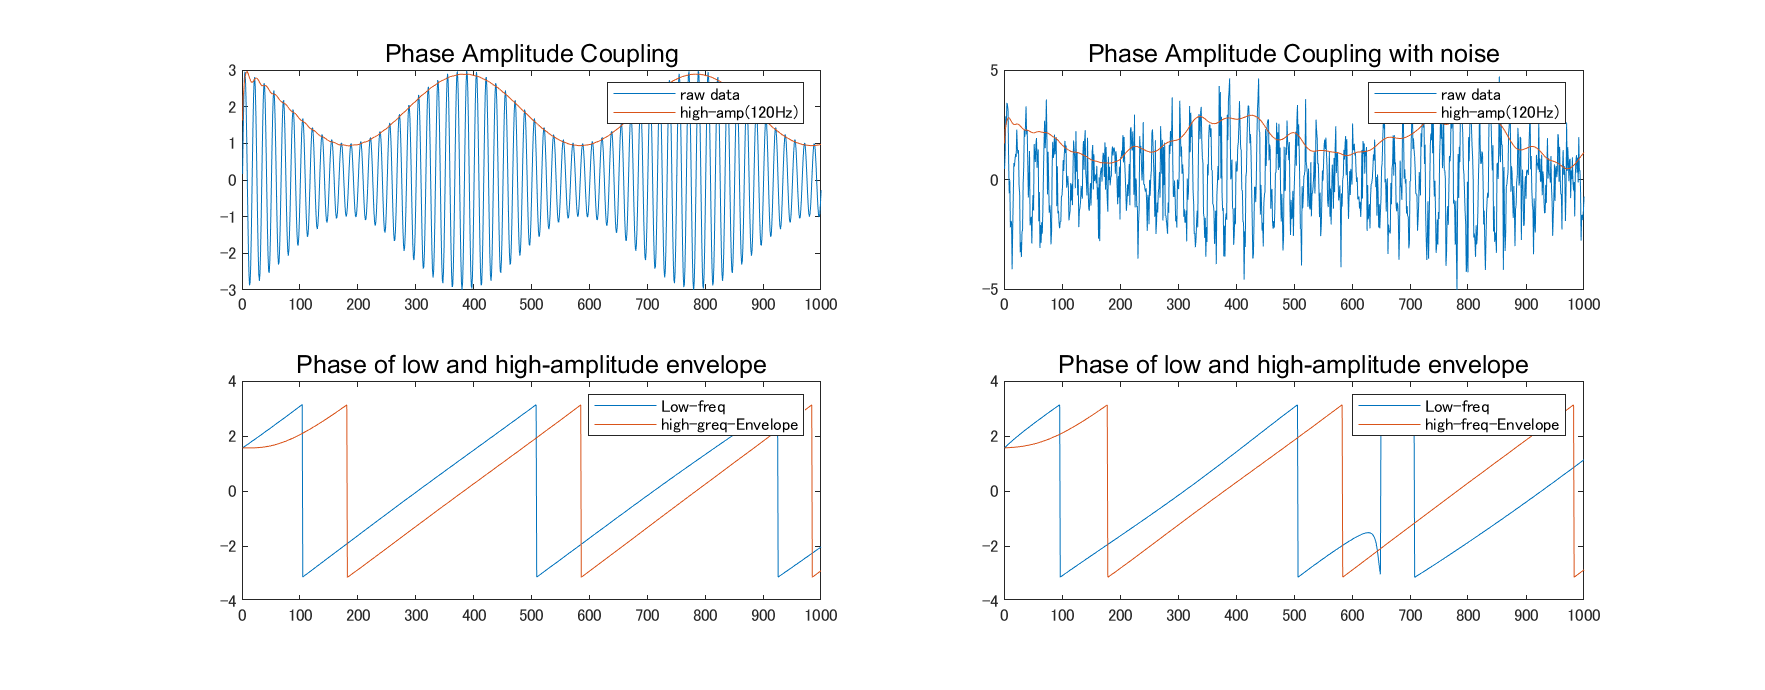
\includegraphics[width=15cm]{../figures/pac.eps}
  \caption{Phase Amplitude Couplingしている波形の例.}
\end{figure}


\subsection{Modulation Index}
\section{部位間同期によるnetwork解析}
こんどかく


\end{document}